\documentclass[11pt, oneside]{article}  % need to compile twice
\usepackage{amsmath, textcomp, amssymb, geometry, graphicx, enumerate, ctex, fancyhdr, float, xcolor}
\usepackage{hyperref}
\usepackage{multirow}
\usepackage{listings}		% 为了避免与页眉的兼容问题可将listings放入table环境中
\lstset{
    basicstyle          =   \sffamily,          % 基本代码风格
    keywordstyle        =   \color{blue},          % 关键字风格
    keywordstyle    =   [2] \color{teal},
    commentstyle        =   \rmfamily\itshape,  % 注释的风格,斜体
    stringstyle         =   \ttfamily,  % 字符串风格
    flexiblecolumns,                % 别问为什么,加上这个
    numbers             =   left,   % 行号的位置在左边
    showspaces          =   false,  % 是否显示空格,显示了有点乱,所以不现实了
    numberstyle         =   \zihao{-5}\ttfamily,    % 行号的样式,小五号,tt等宽字体
    showstringspaces    =   false,
    captionpos          =   t,      % 这段代码的名字所呈现的位置,t指的是top上面
    frame               =   lrtb,   % 显示边框
    basicstyle          =   \zihao{-4}\ttfamily,
    stringstyle         =   \color{magenta},
    commentstyle        =   \color{red}\ttfamily,
    breaklines          =   true,   % 自动换行,建议不要写太长的行
    columns             =   fixed,  % 如果不加这一句,字间距就不固定,很丑,必须加
    basewidth           =   0.5em,
}

\geometry{left=2.54cm, right=2.54cm, top=3.18cm, bottom=3.18cm}

\def\Name{杨豪\space}  % Your name
\def\SID{2206213297}  % Your student ID number

% need to be confirmed before each time writing and committing 
\def\Homework{5} % Number of Homework
\def\Session{2022-Fall}
\def\CourseCodeName{SOFT410911: Software Quality Assurance}
\def\simCourseName{SQA}

\title{\vspace{-4cm}\CourseCodeName \space
        \Session \protect\\  Homework-\textbf{\Homework} Solutions}
\author{软件2101 \Name \space 学号: \SID}
\date{\today}

\markright{\simCourseName\ \space \Session\  HW-\Homework\ \Name}

\begin{document}

\maketitle

\textbf{Honor Code: I promise that I finished the homework solutions on my own without copying other people's work.}

\section*{White-box Testing}

\subsection*{1. Code}

I chose password circumstance of the case used in previous homework solution, QQ register, and wrote a piece of pseudo codes to 
simulate whether input is proper or not.

\begin{lstlisting}[language = Java, 
    caption = {pseudo code for password style check}
    ]
/*
 * A piece of pseudo code for password input correctness checking.
*/
boolean a = b = c = false;
if(input.Contain(' ')) a = false;
else a = true;
if(input.length >= 8 && input.length <= 16) b = true;
else a = false;
if(input.Secure()) c = true;
else c = false;
// Print messages about whether code is proper and why.
PrintMessage(a, b, c);                  
\end{lstlisting}

\subsection*{2. Code Analysis}

After analyze the logic of code above, we can draw a flowchart as below.

\begin{figure}[H]
    \centering
    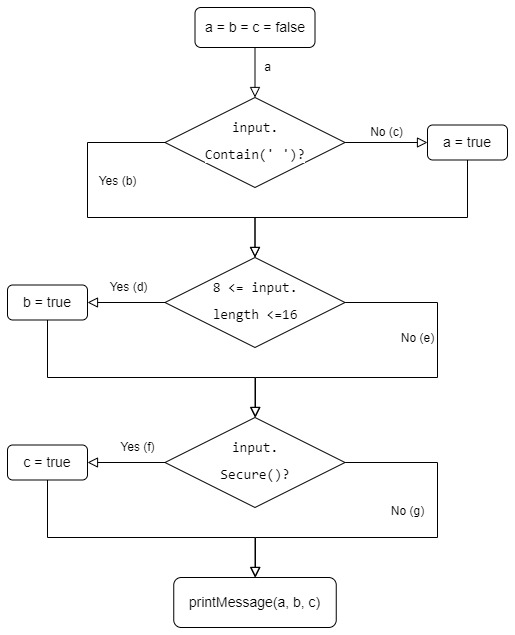
\includegraphics[width = 0.6\textwidth]{./pic/flowchart.jpg}
    \caption{flowchart}
\end{figure}

There are 13 paths in total.

\subsection*{3. Concrete Test Cases}

To simply description, we give conditional judgments short names as below.
\begin{table}[H]
    \begin{tabular}{|c|c|c|c|}
        \hline
        Judgement                     & Short name          & Condition                        & Short name \\ \hline
        input.Contain(' ')?           & P1                  & input.Contain(' ') ?             & C1         \\ \hline
        \multirow{2}{*}{judge.length} & \multirow{2}{*}{P2} & judge.length \textgreater{}= 8 ? & C2         \\ \cline{3-4} 
                                    &                     & judge.length \textless{}= 16 ?   & C3         \\ \hline
        input.Secure()                & P3                  & judge.Secure() ?                 & C4         \\ \hline
    \end{tabular}
\end{table}

\subsubsection*{3.1 Statement coverage}

\begin{table}[H]
    \centering
    \begin{tabular}{|c|c|c|c|c|c|c|c|c|}
    \hline
    Input     & C1 & C2 & C3 & C4 & P1 & P2 & P3 & Path                                              \\ \hline
    12wer?789 &   &   &   &   & F  & T  & T  & a$\rightarrow$c$\rightarrow$d$\rightarrow$f \\ \hline
    \end{tabular}
    \caption{Statement Coverage Case}
\end{table}

\subsubsection*{3.2 Branch coverage}

\begin{table}[H]
    \centering
    \begin{tabular}{|c|c|c|c|c|c|c|c|c|}
        \hline
        Input       & C1 & C2 & C3 & C4 & P1 & P2 & P3 & Path                                              \\ \hline
        12wer?789 &   &   &   &   & F  & T  & T  & a$\rightarrow$c$\rightarrow$d$\rightarrow$f \\ \hline
        1 2       &   &   &   &   & T  & F  & F  & a$\rightarrow$b$\rightarrow$e$\rightarrow$g \\ \hline
    \end{tabular}
    \caption{Branch Coverage Cases}
\end{table}

\subsubsection*{3.3 Condition coverage}

\begin{table}[H]
    \centering
    \begin{tabular}{|c|c|c|c|c|c|c|c|c|}
        \hline
        Input                & C1 & C2 & C3 & C4 & P1 & P2 & P3 & Path                                              \\ \hline
        12wer?789          & F  & T  & T  & T  &   &   &   & a$\rightarrow$c$\rightarrow$d$\rightarrow$f \\ \hline
        1 2                & T  & F  & T  & F  &   &   &   & a$\rightarrow$b$\rightarrow$e$\rightarrow$g \\ \hline
        123abc456def789efg & F  & T  & F  & T  &   &   &   & a$\rightarrow$c$\rightarrow$e$\rightarrow$f \\ \hline
    \end{tabular}
    \caption{Condition Coverage Cases}
\end{table}

\subsubsection*{3.4 Decision-Condition coverage}

\begin{table}[H]
    \centering
    \begin{tabular}{|c|c|c|c|c|c|c|c|c|}
    \hline
    Input                & C1 & C2 & C3 & C4 & P1 & P2 & P3 & Path                                              \\ \hline
    12wer?789          & F  & T  & T  & T  & F  & T  & T  & a$\rightarrow$c$\rightarrow$d$\rightarrow$f \\ \hline
    1 2                & T  & F  & T  & F  & T  & F  & F  & a$\rightarrow$b$\rightarrow$e$\rightarrow$g \\ \hline
    123abc456def789efg & F  & T  & F  & T  & F  & F  & T  & a$\rightarrow$c$\rightarrow$e$\rightarrow$f \\ \hline
    \end{tabular}
    \caption{Decision-Condition Coverage Cases}
\end{table}

\subsubsection*{3.5 Condition combinatorial coverage}

\begin{table}[H]
    \centering
    \begin{tabular}{|c|c|c|c|c|c|c|c|c|}
    \hline
        Input              & C1 & C2 & C3 & C4 & P1 & P2 & P3 & Path                                              \\ \hline
        eq213 456          & T  & T  & T  & T  &    &    &    & a$\rightarrow$b$\rightarrow$d$\rightarrow$f \\ \hline
        12345 456          & T  & T  & T  & F  &    &    &    & a$\rightarrow$b$\rightarrow$d$\rightarrow$g \\ \hline
        qwbw1098 89asbb?-  & T  & T  & F  & T  &    &    &    & a$\rightarrow$b$\rightarrow$e$\rightarrow$f \\ \hline
        00000000 000000000 & T  & T  & F  & F  &    &    &    & a$\rightarrow$b$\rightarrow$e$\rightarrow$g \\ \hline
        @1 q?              & T  & F  & T  & T  &    &    &    & a$\rightarrow$b$\rightarrow$e$\rightarrow$f \\ \hline
        1 2                & T  & F  & T  & F  &    &    &    & a$\rightarrow$b$\rightarrow$e$\rightarrow$g \\ \hline
        12wer?789          & F  & T  & T  & T  &    &    &    & a$\rightarrow$c$\rightarrow$d$\rightarrow$f \\ \hline
        12345678           & F  & T  & T  & F  &    &    &    & a$\rightarrow$c$\rightarrow$d$\rightarrow$g \\ \hline
        123abc456def789efg & F  & T  & F  & T  &    &    &    & a$\rightarrow$c$\rightarrow$e$\rightarrow$f \\ \hline
        00000000000000000  & F  & T  & F  & F  &    &    &    & a$\rightarrow$c$\rightarrow$e$\rightarrow$g \\ \hline
        @1q?Q2             & F  & F  & T  & T  &    &    &    & a$\rightarrow$c$\rightarrow$e$\rightarrow$f \\ \hline
        000000             & F  & F  & T  & F  &    &    &    & a$\rightarrow$c$\rightarrow$e$\rightarrow$g \\ \hline
    \end{tabular}
    \caption{Condition Combinatorial Coverage Cases}
\end{table}

\subsubsection*{3.6 Path coverage}

\begin{table}[H]
    \centering
    \begin{tabular}{|c|c|c|c|c|c|c|c|c|}
    \hline
    Input              & C1 & C2 & C3 & C4 & P1 & P2 & P3 & Path                                              \\ \hline
    eq213 456          &    &    &    &    & T  & T  & T  & a$\rightarrow$b$\rightarrow$d$\rightarrow$f \\ \hline
    12345 456          &    &    &    &    & T  & T  & F  & a$\rightarrow$b$\rightarrow$d$\rightarrow$g \\ \hline
    qwbw1098 89asbb?-  &    &    &    &    & T  & F  & T  & a$\rightarrow$b$\rightarrow$e$\rightarrow$f \\ \hline
    00000000 000000000 &    &    &    &    & T  & F  & F  & a$\rightarrow$b$\rightarrow$e$\rightarrow$g \\ \hline
    12wer?789          &    &    &    &    & F  & T  & T  & a$\rightarrow$c$\rightarrow$d$\rightarrow$f \\ \hline
    12345678           &    &    &    &    & F  & T  & F  & a$\rightarrow$c$\rightarrow$d$\rightarrow$g \\ \hline
    123abc456def789efg &    &    &    &    & F  & F  & T  & a$\rightarrow$c$\rightarrow$e$\rightarrow$f \\ \hline
    00000000000000000  &    &    &    &    & F  & F  & F  & a$\rightarrow$c$\rightarrow$e$\rightarrow$g \\ \hline
    \end{tabular}
    \caption{Path Coverage Cases}
\end{table}

\subsection*{4. Summary}

It's easy to realize that the Condition Combinatorial Coverage Cases can cover other tests, which leads to his huge amount of 
tets cases. Other coverage may have less cases, but they always neglect some likelihood. 
In real world, we have to trade off between amount of cases and coverage percentage.

\section*{Other things}

    \LaTeX \space code refer to these things and was complied on texlive2020 by \lstinline{xelatex}.
    \begin{itemize}
        \item  \href{https://www.eecs70.org/assets/misc/homework_template.tex}{UCB-CS70's given homework template.} 
        \item  \href{https://www.tablesgenerator.com/}{A free website useful to edit \LaTeX \space table code.}
    \end{itemize}

    The purpose of writing in English is to adapt to bilingual teaching and to improve my poor English 
    writing skills in preparation for a possible future exchange program. 

    Thanks for your correcting and grading :).

\end{document}

 
